\documentclass[11pt,a4paper]{article}
\usepackage[margin=2.3cm]{geometry}
\usepackage{amsmath,amssymb,amsthm}
\usepackage{graphicx}
\usepackage{booktabs}
\usepackage{siunitx}
\usepackage{caption}
\usepackage{algorithm}
\usepackage{algpseudocode}
\usepackage[numbers,sort&compress]{natbib}
\usepackage{hyperref}
\usepackage{cleveref}
\graphicspath{{figures/}}
\setlength{\emergencystretch}{4em}

\newtheorem{proposition}{Proposition}
\newtheorem{theorem}{Theorem}
\newtheorem{lemma}{Lemma}
\newtheorem{corollary}{Corollary}
\theoremstyle{remark}
\newtheorem{remark}{Remark}

\newcommand{\dd}{\mathrm{d}}
\newcommand{\rt}{\tilde\rho}
\newcommand{\het}{\nu}
\newcommand{\etab}{\eta_{b}}
\newcommand{\etal}{\eta_{\ell}}
\newcommand{\pd}{\partial}

\title{Orthogonal terrain-following coordinates for the rational\\
one-way Helmholtz equation:\\
irregular terrain and bathymetry without staircases, angle limits\\
or changes to the discrete nonlocal boundary condition}
\author{Mikhail S.\ Lytaev}
\date{\today}

\begin{document}
\maketitle

\begin{abstract}
Irregular terrain in tropospheric propagation and irregular bathymetry in
underwater acoustics are usually represented in finite-difference parabolic
equation (PE) solvers by staircases. We replace the staircase by a change of
variables that maps the physical domain onto a rectangle. The map is required
to (i) leave the Helmholtz operator in a form to which a rational
(Pad\'e, rational-interpolation) approximation of the one-way propagator of
\emph{arbitrary} order applies unchanged, so that no restriction on the
propagation angle is introduced; and (ii) be the identity near the artificial
boundary, so that the discrete nonlocal transparent boundary condition (NLBC)
is used without modification. We show that sheared (Beilis--Tappert) coordinates
cannot satisfy (i): the incident and reflected vertical wavenumbers at the
boundary are not symmetric, so no function of the vertical operator reproduces
the reflection. Conformal maps satisfy (i) but, by the identity theorem, cannot
satisfy (ii). Orthogonal but non-conformal coordinates satisfy both. We
construct them from the harmonic extension of the boundary, tapered to the
identity, and from the orthogonal trajectories of the resulting family of level
curves. In these coordinates the Helmholtz equation becomes a Sturm--Liouville
problem with a generalised density $\rt=\rho h_\eta/h_\xi$ and a weight $m=(h_\eta/h_\xi)^2$.
Each factor of the rational propagator then reduces to the density-weighted
Numerov scheme with one extra diagonal weight. Range dependence of the metric
is handled by a Liouville transformation and by a flux-conserving step
$B_{n+1}^{-1/4}R B_n^{1/4}$. We write this step in a form that is the identity
in the exterior, so the NLBC of the plain rational chain still applies. A
discrete dispersion analysis shows that the transformed scheme is locally
\emph{equivalent} to the untransformed one on a grid with steps
$h_\xi\Delta\xi$, $h_\eta\Delta\eta$ and reference wavenumber $\beta/h_\xi$. Hence
the existing grid optimizer applies after a rescaling of its inputs, and the
angle limit is the one of the chosen rational approximation, measured from the
local marching direction. The method is implemented in JAX in
\texttt{pywaveprop}. Against an exact solution for a beam reflected by a
perfectly conducting slope (reflected beam up to $70^\circ$) its error is two to
three orders of magnitude below that of the staircase. It agrees with a
finely resolved RAM solution for a penetrable wedge. It is demonstrated on
real terrain (SRTM-type elevation data) and real bathymetry and Argo sound
speed profiles.
\end{abstract}

\tableofcontents

%=====================================================================
\section{Introduction}\label{sec:intro}

\texttt{pywaveprop} solves the one-way (pseudo-differential parabolic) Helmholtz
equation with a rational approximation of the propagator,
\begin{equation}\label{eq:rational}
\exp\!\bigl(i\beta\Delta x(\sqrt{1+L}-1)\bigr)\approx R(L)=\prod_{l=1}^{p}\frac{1+a_lL}{1+b_lL},
\end{equation}
a fourth-order (Numerov-type) vertical discretisation of $L$
\cite{lytaev2020awpl}, an automated selection of $\Delta x$, $\Delta z$, $\beta$ and
of the order \cite{lytaev2020iccsa,lytaev2023jmse,lytaev2026nmp}, and the
discrete NLBC at the upper (troposphere) or lower (ocean bottom) artificial
boundary \cite{lytaev2018awpl}. Terrain and bathymetry are represented by a
staircase: the field is set to zero below the terrain (or below the seabed)
column by column. A staircase converges only at first order in $\Delta z$, it
generates spurious diffraction at every step, it cannot represent a
penetrable sloping interface with the correct continuity conditions, and for
steep slopes it requires a vertical step much smaller than the one dictated by
the propagation angle.

The aim of this note is a change of variables that maps the physical domain
onto a rectangle, with the irregular boundary becoming a coordinate line, under
three constraints:
\begin{enumerate}
\item no restriction on the maximum propagation angle is introduced: any angle
that the rational approximation \eqref{eq:rational} resolves on flat ground is
resolved over terrain, for an approximation of \emph{arbitrary} order;
\item the upper discrete NLBC is used without modification;
\item the formulation covers both tropospheric radio-wave propagation
(impenetrable terrain) and underwater acoustics (penetrable seabed with a
density jump).
\end{enumerate}

\subsection{Related work}\label{sec:review}

A literature survey (180 references, 42 of them available as PDFs; the list
with DOIs is in \texttt{refs/README.md}) gives the following picture.

\paragraph{Shift maps.}
The Beilis--Tappert transformation $\zeta=z-T(x)$ \cite{beilis1979coupled},
together with a phase factor $e^{ikT'\zeta+\frac{ik}{2}\int T'^2}$, maps the
\emph{narrow-angle} PE over terrain exactly onto the PE over flat ground with an
additional potential $-2k^2\zeta T''$. It is the basis of TPEM, TEMPER and APM
\cite{barrios1994tpem,donohue2000gtpe,barrios2003apm}, of the acoustic
PERUSE model \cite{dozier1984peruse} and of many later terrain PE codes
\cite{parakkal2012beilis,khodr2020iterative,wang2020smpe}. In the Helmholtz
equation, however, the shear produces the mixed derivative $-2T'\pd_x\pd_\zeta$,
and the phase factor removes it only at the paraxial level. Wide-angle variants
\cite{donohue2000gtpe} split the square-root operator to first order in the
slope. Published limits are about $10$--$20^\circ$ for slopes, and the slope
error is not reduced by raising the Pad\'e order \cite{wang2020smpe}.

\paragraph{Rotations and mapped depth coordinates.}
The rotated PE \cite{collins1990rotated,outing2006variable} is exact (the Laplacian
is rotation invariant) and works with any Pad\'e order, but only for
piecewise-constant slopes; the field has to be interpolated at every slope
break. Depth scalings $y=z/D(x)$
\cite{abrahamsson1990bc,akrivis1994galerkin,collins2000mapping,metzler2014scaled}
and the curvilinear scheme of Janaswamy \cite{janaswamy1998curvilinear} are
applied to an already paraxial equation, so each order needs a new derivation.
Collins' energy-conserving \cite{collins1991energy} and single-scattering
corrections improve the staircase interface conditions but keep the staircase.

\paragraph{Conformal and orthogonal maps.}
A conformal map $x+iz=F(\xi+i\eta)$ preserves the Laplacian, so the Helmholtz
equation becomes the Helmholtz equation with index $n^2|F'|^2$. Dirichlet and
Neumann conditions are invariant and the divergence form with density is
preserved. Conformal maps were used for terrain and rough surfaces with
\emph{narrow-angle} split-step Fourier solvers
\cite{dozier1984peruse,donohue1997apl}, for bent optical waveguides
\cite{heiblum1975conformal}, and for water waves with wide-angle rational PEs
\cite{kirby1994conformal}. The Earth-flattening transformation is the
best-known example. Local orthogonal transformations combined with exact one-way
(Dirichlet-to-Neumann) methods were developed by Lu and co-workers for bounded
acoustic waveguides \cite{lu1999exact,lu2001lot,lu2004lot}; the equation they
obtain has the same structure as ours, but no transparent boundary is involved.

\paragraph{Transparent boundaries.}
All exact discrete transparent boundary conditions
\cite{arnold_ehrhardt1998jcp,ehrhardt_zisowsky2007,lytaev2018awpl,lytaev2022radarconf}
assume an exterior whose coefficients do not depend on range. Kampanis
\cite{kampanis2002,kampanis2005} used a terrain-fitting map that is the identity
near the top boundary, so that the NLBC is unaffected, but with a narrow-angle
finite-element PE; such maps are not conformal and produce mixed derivatives.

\paragraph{Gap.} No published method combines a Helmholtz-exact map of the
irregular boundary, an arbitrary-order rational propagator, and an exact
discrete NLBC. The closest precedents combine two of the three:
Earth flattening with \cite{lytaev2018awpl}, Kampanis's mapped finite elements
with an NLBC, and Kirby's wide-angle PE in conformal coordinates. This note fills
the gap.

\subsection{Contributions and outline}

\Cref{sec:why} explains which maps are compatible with the rational propagator:
sheared coordinates are not (\cref{prop:shear}), orthogonal coordinates are
(\cref{prop:orth}), and conformal coordinates cannot be the identity near the
NLBC (\cref{prop:conformal}). \Cref{sec:map} constructs orthogonal coordinates
that are the identity in the exterior. \Cref{sec:transformed} derives the
transformed one-way equation, including the Liouville and flux-conserving
treatment of the range dependence of the metric. \Cref{sec:disc} gives the
discretisation, \cref{sec:dispersion} the discrete dispersion analysis,
\cref{sec:nlbc} the compatibility with the NLBC, \cref{sec:impl} the
implementation, and
\cref{sec:validation,sec:realdata} the validation and the real-data
demonstrations.

%=====================================================================
\section{Problem statement}\label{sec:problem}

We consider the two-dimensional Helmholtz equation for a time-harmonic field
$\psi(x,z)$ (time dependence $e^{-i\omega t}$),
\begin{equation}\label{eq:helmholtz}
\rho\,\nabla\cdot\bigl(\rho^{-1}\nabla\psi\bigr)+k^2(x,z)\,\psi=0,\qquad k=\frac{\omega}{c}\,(1+i\eta_\alpha\alpha),
\end{equation}
with $\rho\equiv1$ in tropospheric propagation ($k^2=k_0^2n^2$, $n$ including
the Earth-flattening term of the modified refractivity $M$).
\begin{itemize}
\item \textbf{Troposphere.} $z$ is the height above sea level, the domain is
$\Omega=\{z>T(x)\}$, $T$ is the terrain, and the ground is perfectly conducting:
$\psi=0$ (horizontal polarisation) or $\pd_n\psi=0$ (vertical polarisation) on
$z=T(x)$.
\item \textbf{Ocean.} $z$ is the depth, the sea surface $z=0$ is pressure
release ($\psi=0$), and the seabed $z=T(x)$ separates the water (density
$\rho_w$, sound speed $c_w(z)$) from a fluid bottom ($\rho_b$, $c_b$,
attenuation $\alpha_b$). On it $[\psi]=0$ and $[\rho^{-1}\pd_n\psi]=0$.
\end{itemize}
In both cases the field radiates through the outer side of the domain (up in
the troposphere, down in the ocean bottom), where the medium does not depend on
$x$ and is homogeneous or has a linear $k^2(z)$ (standard atmosphere). There
the domain is truncated by the discrete NLBC.

\paragraph{The rational one-way propagator.}
On flat ground, with $L=\beta^{-2}(\rho\pd_z\rho^{-1}\pd_z+k^2)-1$ and the
envelope $u=\psi e^{-i\beta x}$, the outgoing part of $\psi$ satisfies
$u_x=i\beta(\sqrt{1+L}-1)u$, and one range step is \eqref{eq:rational}.
Each factor is a tridiagonal solve
\begin{equation}\label{eq:substep_flat}
b_l\,\delta^2_\rho v+(1+\alpha\delta_\rho^2)\bigl[\tau^2(1+b_l\het)v\bigr]=
a_l\,\delta^2_\rho u+(1+\alpha\delta_\rho^2)\bigl[\tau^2(1+a_l\het)u\bigr],
\end{equation}
with $\tau=\beta\Delta z$, $\alpha=1/12$, $\het=k^2/\beta^2-1$ and the
density-weighted second difference
\[
\delta^2_\rho u_j=\rho_j\Bigl(\frac{u_{j+1}-u_j}{\rho_{j+1/2}}-\frac{u_j-u_{j-1}}{\rho_{j-1/2}}\Bigr).
\]
For $\rho\equiv1$ this is the Numerov--Pad\'e scheme of \cite{lytaev2020awpl}.
The discrete NLBC \cite{lytaev2018awpl} expresses the last unknown of every
factor through the history of the boundary values of all factors,
\begin{equation}\label{eq:nlbc}
u^{n}_{N-1,l}-Q^{(0)}_{ll}u^{n}_{N,l}=\sum_{m=1}^{n}\sum_{l'}Q^{(m)}_{ll'}u^{n-m}_{N,l'}+\sum_{l'<l}Q^{(0)}_{ll'}u^n_{N,l'},
\end{equation}
where the kernels $Q^{(m)}$ are the inverse $z$-transform of a matrix function
built from the coefficients $a_l$, $b_l$ and from the discrete exterior
equation. They depend only on the exterior scheme and on the chain of factors.

%=====================================================================
\section{Which changes of variables are compatible with the rational propagator}\label{sec:why}

A rational propagator of arbitrary order needs the one-way operator to be a
function of a single vertical operator, $\exp(i\Delta\xi\sqrt{B})$. On flat
ground with a Dirichlet boundary this is the case because the incident and
reflected vertical wavenumbers are $\pm q$, the eigenfunctions $\sin q\eta$ of
the Dirichlet operator $\pd_\eta^2$.

\begin{proposition}[sheared coordinates]\label{prop:shear}
Let $\zeta=z-sx$ with constant $s=\tan\theta_s$, $k$ constant, and $\psi=0$ on
$\zeta=0$. The time-harmonic solutions $e^{ipx}f(\zeta)$ are
$f=e^{iq_+\zeta}-e^{iq_-\zeta}$ with
\begin{equation}\label{eq:qpm}
q_\pm=\frac{sp\pm\sqrt{(1+s^2)k^2-p^2}}{1+s^2},\qquad q_++q_-=\frac{2sp}{1+s^2}\ne0 .
\end{equation}
Hence for $s\ne0$ the exact forward propagator in $x$ does not commute with the
Dirichlet realisation of $\pd^2_\zeta$, and no propagator of the form
$G(x)\,F(\pd_\zeta^2)$ with a multiplicative gauge $G$ is exact for all $p$.
The Beilis--Tappert gauge $G=e^{iks\zeta}$ symmetrises the pair only if
$p=k(1+s^2)$, a value that propagating waves never reach since
$p\le k\sqrt{1+s^2}$. For a wave at the angle $\alpha$ to the $x$ axis the
remaining asymmetry is
\[
\frac{q_++q_--2ks}{k}=2s\bigl(\cos(\alpha-\theta_s)\cos\theta_s-1\bigr).
\]
\end{proposition}
\begin{proof}
Substituting $\psi=e^{ipx+iq\zeta}$ into
$\psi_{xx}-2s\psi_{x\zeta}+(1+s^2)\psi_{\zeta\zeta}+k^2\psi=0$ gives
$(1+s^2)q^2-2spq+p^2-k^2=0$, whence \eqref{eq:qpm}. A wave
$e^{i(k_xx+k_zz)}$ has $p=k_x+sk_z$; inserting $k_x=k\cos\alpha$,
$k_z=k\sin\alpha$ gives the last formula.
\end{proof}
The asymmetry is $O(\theta_s^3)$ at grazing incidence on the slope, which is why
the shift map works paraxially, and $O(\theta_s)$ otherwise
(\cref{fig:shear}). It does not decrease with the order of the rational
approximation.

\begin{figure}[t]\centering
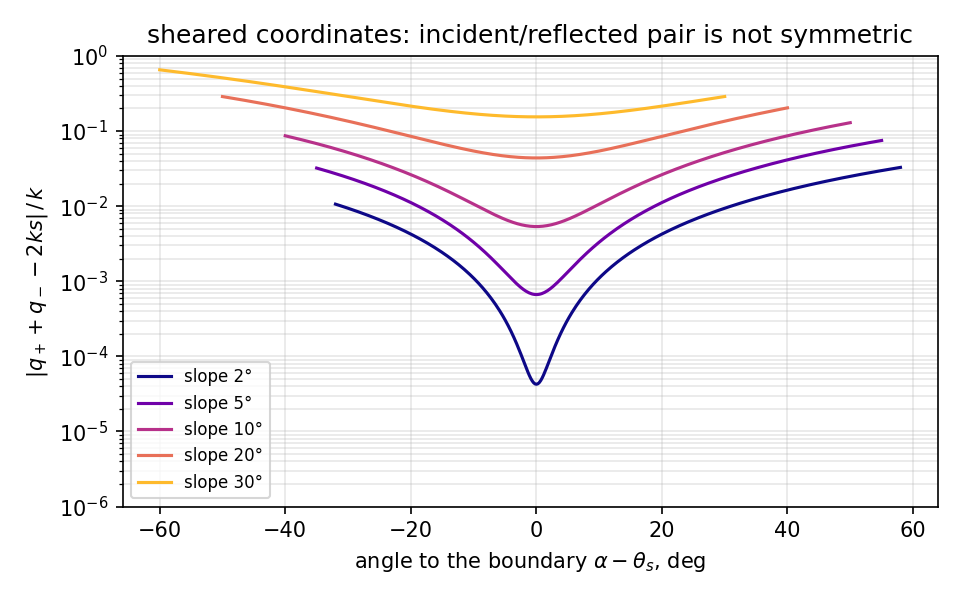
\includegraphics[width=0.62\textwidth]{disp_shear_asymmetry.png}
\caption{Asymmetry of the incident/reflected pair of vertical wavenumbers in
sheared coordinates after the Beilis--Tappert gauge (\cref{prop:shear}).}
\label{fig:shear}
\end{figure}

\begin{proposition}[orthogonal coordinates]\label{prop:orth}
Let $(\xi,\eta)$ be orthogonal coordinates with scale factors $h_\xi$,
$h_\eta$ and $r=h_\eta/h_\xi$. Then \eqref{eq:helmholtz} reads
\begin{equation}\label{eq:helm_orth}
\pd_\xi\Bigl(\frac{r}{\rho}\pd_\xi\psi\Bigr)+\pd_\eta\Bigl(\frac{1}{r\rho}\pd_\eta\psi\Bigr)+\frac{h_\xi h_\eta}{\rho}k^2\psi=0,
\end{equation}
without a mixed derivative. For frozen $h_\xi$, $h_\eta$ the reflection
$\eta\mapsto-\eta$ is a symmetry of \eqref{eq:helm_orth}. Hence the
Dirichlet (Neumann) half-space solutions are odd (even) images, the incident and
reflected wavenumbers are $\pm q$, and the exact forward propagator is
$\exp\bigl(i\Delta\xi\sqrt{B}\bigr)$ with $B=h_\xi^2k^2+r^{-2}\pd^2_\eta$
realised with the boundary condition.
\end{proposition}
\begin{proof}
In orthogonal coordinates
$\nabla\cdot(a\nabla\psi)=(h_\xi h_\eta)^{-1}\bigl[\pd_\xi(ah_\eta h_\xi^{-1}\pd_\xi\psi)+\pd_\eta(ah_\xi h_\eta^{-1}\pd_\eta\psi)\bigr]$;
multiply by $h_\xi h_\eta/\rho$. With frozen coefficients the equation is
$r\psi_{\xi\xi}+r^{-1}\psi_{\eta\eta}+h_\xi h_\eta k^2\psi=0$, even in $\eta$.
\end{proof}

So orthogonality, not conformality, is what the rational propagator needs. A
conformal map is the special case $r\equiv1$. It cannot be used here because of
the following fact.

\begin{proposition}[conformal maps and the NLBC]\label{prop:conformal}
Let $F$ be analytic in a connected domain $W$ and $F(w)=w+c$ on an open subset
of $W$. Then $F(w)=w+c$ on all of $W$. Consequently a conformal map that
straightens a non-flat boundary is not the identity (up to a shift) in any open
set, in particular not near the NLBC; there $|F'|^2\ne1$, and the exterior index
$n^2|F'|^2$ depends on range.
\end{proposition}
\begin{proof}
Identity theorem for analytic functions.
\end{proof}

For a strip or periodic conformal map $|F'|^2-1$ decays like
$e^{-2\pi\eta/\ell}$, where $\ell$ is the horizontal scale of the terrain. For a
terrain feature \SI{10}{km} long the residual is still $O(10^{-1})$ at a height
of \SI{1}{km}, and the NLBC kernel would see a range-dependent exterior. We
therefore give up conformality and keep orthogonality.

%=====================================================================
\section{Construction of the map}\label{sec:map}

\subsection{Family of level curves}

The coordinate lines $\eta=\mathrm{const}$ are the curves $z=Z(x,\eta)$ with
\begin{equation}\label{eq:family}
Z(x,\eta)=\eta+z_{\rm off}+u(x,\eta),
\end{equation}
where $u$ is the harmonic extension of the boundary, tapered to zero. Let
$b(x)=T(x)-z_{\rm off}-\etab$ and $\hat b(\kappa)$ its Fourier transform. With
$t=(\eta-\etab)/L$,
\begin{equation}\label{eq:kernel}
\hat u(\kappa,\eta)=\hat b(\kappa)\times
\begin{cases}
\eta/\etab\quad\Bigl(\text{or }\dfrac{\sinh\kappa\eta}{\sinh\kappa\etab}\Bigr), & 0\le\eta<\etab\quad\text{(strip, ocean)},\\[2ex]
w(t)\,e^{-|\kappa|(\eta-\etab)}, & \eta\ge\etab,
\end{cases}
\end{equation}
with the $C^2$ taper $w(t)=1-t^3(10-15t+6t^2)$ for $0\le t\le1$ and $w=0$ for
$t\ge1$.
\begin{itemize}
\item \textbf{Troposphere (half-space map).} $\etab=0$, $z_{\rm off}=z_{\rm ref}$.
The terrain is the line $\eta=0$ and the coordinates relax to $z=\eta+z_{\rm ref}$.
\item \textbf{Ocean (strip map).} $z_{\rm off}=0$, $\etab=\max T$. The surface
$z=0$ is $\eta=0$, the seabed is $\eta=\etab$, and the coordinates are
$z=\eta$ deep in the bottom.
\end{itemize}
The family has the following properties.
\begin{enumerate}
\item $Z(x,\etab)=T(x)$ exactly, and in the strip $Z(x,0)=0$.
\item \emph{Identity region}: $Z=\eta+z_{\rm off}$ for $\eta\ge\etal=\etab+L$.
\item Above the boundary, near it ($w\approx1$), $u$ is harmonic. A feature of
horizontal scale $\ell$ decays over a height $\sim\ell$, so small-scale relief is
confined near the boundary, as with a conformal map, and only the large-scale
relief reaches the taper.
\item In the water column the default is the $\sigma$-coordinate
$Z=\eta T(x)/\etab$, with $Z_\eta=T/\etab>0$ for any bathymetry. The harmonic
($\sinh$) profile keeps the near-conformal property, but the $\eta$-derivative
of the strip kernel has negative lobes. Next to steep, high relief it then
overshoots and makes $Z_\eta<0$: on the Bermuda pedestal (\cref{sec:realdata})
this happens for every smoothing width up to \SI{1}{km}.
\item \emph{Regularity}: the map is invertible if $Z_\eta>0$. In the water column
of the strip map $Z_\eta=T/\etab>0$. Above $\etab$ write $u=w(t)U$, where $U$ is
the (Poisson) harmonic extension of $b$, so that
\[
Z_\eta=1+w\,U_\eta+\frac{w'}{L}\,U .
\]
\begin{itemize}
\item With $z_{\rm ref}=\max T$ (or $\etab=\max T$), $b\le0$, hence $U\le0$ by the
maximum principle, and $w'\le0$, so the taper term is non-negative and
$Z_\eta\ge1-\max|U_\eta|$ for every $L$. Here $U_\eta=\mathcal H[b']$ at the
boundary is a bound on the (smoothed) slopes.
\item With $z_{\rm ref}=\overline T$ the taper compresses the high parts, and
$Z_\eta\ge1-\max|U_\eta|-\tfrac{15}{8}\max(T-z_{\rm ref})/L$.
\end{itemize}
The implementation checks $Z_\eta>0$ (and $h_\xi>0$) numerically and falls back
to $z_{\rm ref}=\max T$.
\end{enumerate}

The boundary is extended evenly at $x=0$ and at the far end of a padded
interval, and is filtered with a Gaussian of width $\sigma$ (removing the corners
of the piecewise-linear elevation samples). The even extension makes $u_x(0,\eta)=0$,
so the starting trajectory $\xi=0$ is the vertical line $x=0$ and the source
aperture can be prescribed as a function of height, as on flat ground.

\subsection{Orthogonal trajectories}

Let $X(\xi,\eta)$ be the abscissa of the trajectory orthogonal to the level
curves that leaves the identity region at $x=\xi$:
\begin{equation}\label{eq:traj}
\frac{\pd X}{\pd\eta}=G(X,\eta)\equiv-\frac{Z_xZ_\eta}{1+Z_x^2},\qquad X(\xi,\etal)=\xi .
\end{equation}
The tangent of the trajectory, $(X_\eta,\ Z_xX_\eta+Z_\eta)$, is orthogonal to the
tangent $(1,Z_x)$ of the level curve:
$X_\eta(1+Z_x^2)+Z_xZ_\eta=0$. The map is $(\xi,\eta)\mapsto(X,Z(X,\eta))$.
Trajectories are integral curves of the smooth vector field $\nabla\eta$, which
does not vanish because $Z_\eta>0$, so they never cross. The scale factors are
\begin{equation}\label{eq:metric}
h_\eta=\frac{Z_\eta}{\sqrt{1+Z_x^2}},\qquad h_\xi=P\sqrt{1+Z_x^2},\qquad
P=\frac{\pd X}{\pd\xi},\quad \frac{\pd P}{\pd\eta}=G_x(X,\eta)\,P,\ \ P(\xi,\etal)=1,
\end{equation}
since $h_\eta^2=X_\eta^2+(Z_xX_\eta+Z_\eta)^2=Z_\eta^2/(1+Z_x^2)$ and
$\pd_\xi(X,Z(X,\eta))=P(1,Z_x)$. In the identity region $h_\xi=h_\eta=r=1$. At the
level $\etab$ of the strip map the family is only continuous, so $h_\eta$ and
$r$ jump while $h_\xi$ stays continuous. This jump is harmless because the
seabed is a density interface anyway (\cref{sec:transformed}).

\paragraph{Numerical construction.} $\hat b$ is computed once by FFT on a
uniform grid. For every level needed by the integrator, $u$, $u_x$, $u_{xx}$,
$u_\eta$, $u_{x\eta}$ are evaluated by five inverse FFTs. The system
\eqref{eq:traj}--\eqref{eq:metric} is integrated downwards from $\etal$ with
RK4 for all columns simultaneously, on coarse levels with spacing about
$\sigma/8$ placed separately on $[0,\etab]$ and $[\etab,\etal]$. The metrics are
then interpolated to the computational nodes and half-nodes with cubic splines
on each side of $\etab$. The orthogonality and the metric formulas were checked
against finite differences of the computed $(X,Z)$: the cosine of the angle
between the coordinate lines is below $2\cdot10^{-4}$, at the level of the
finite-difference error of the check.

\begin{figure}[p]\centering
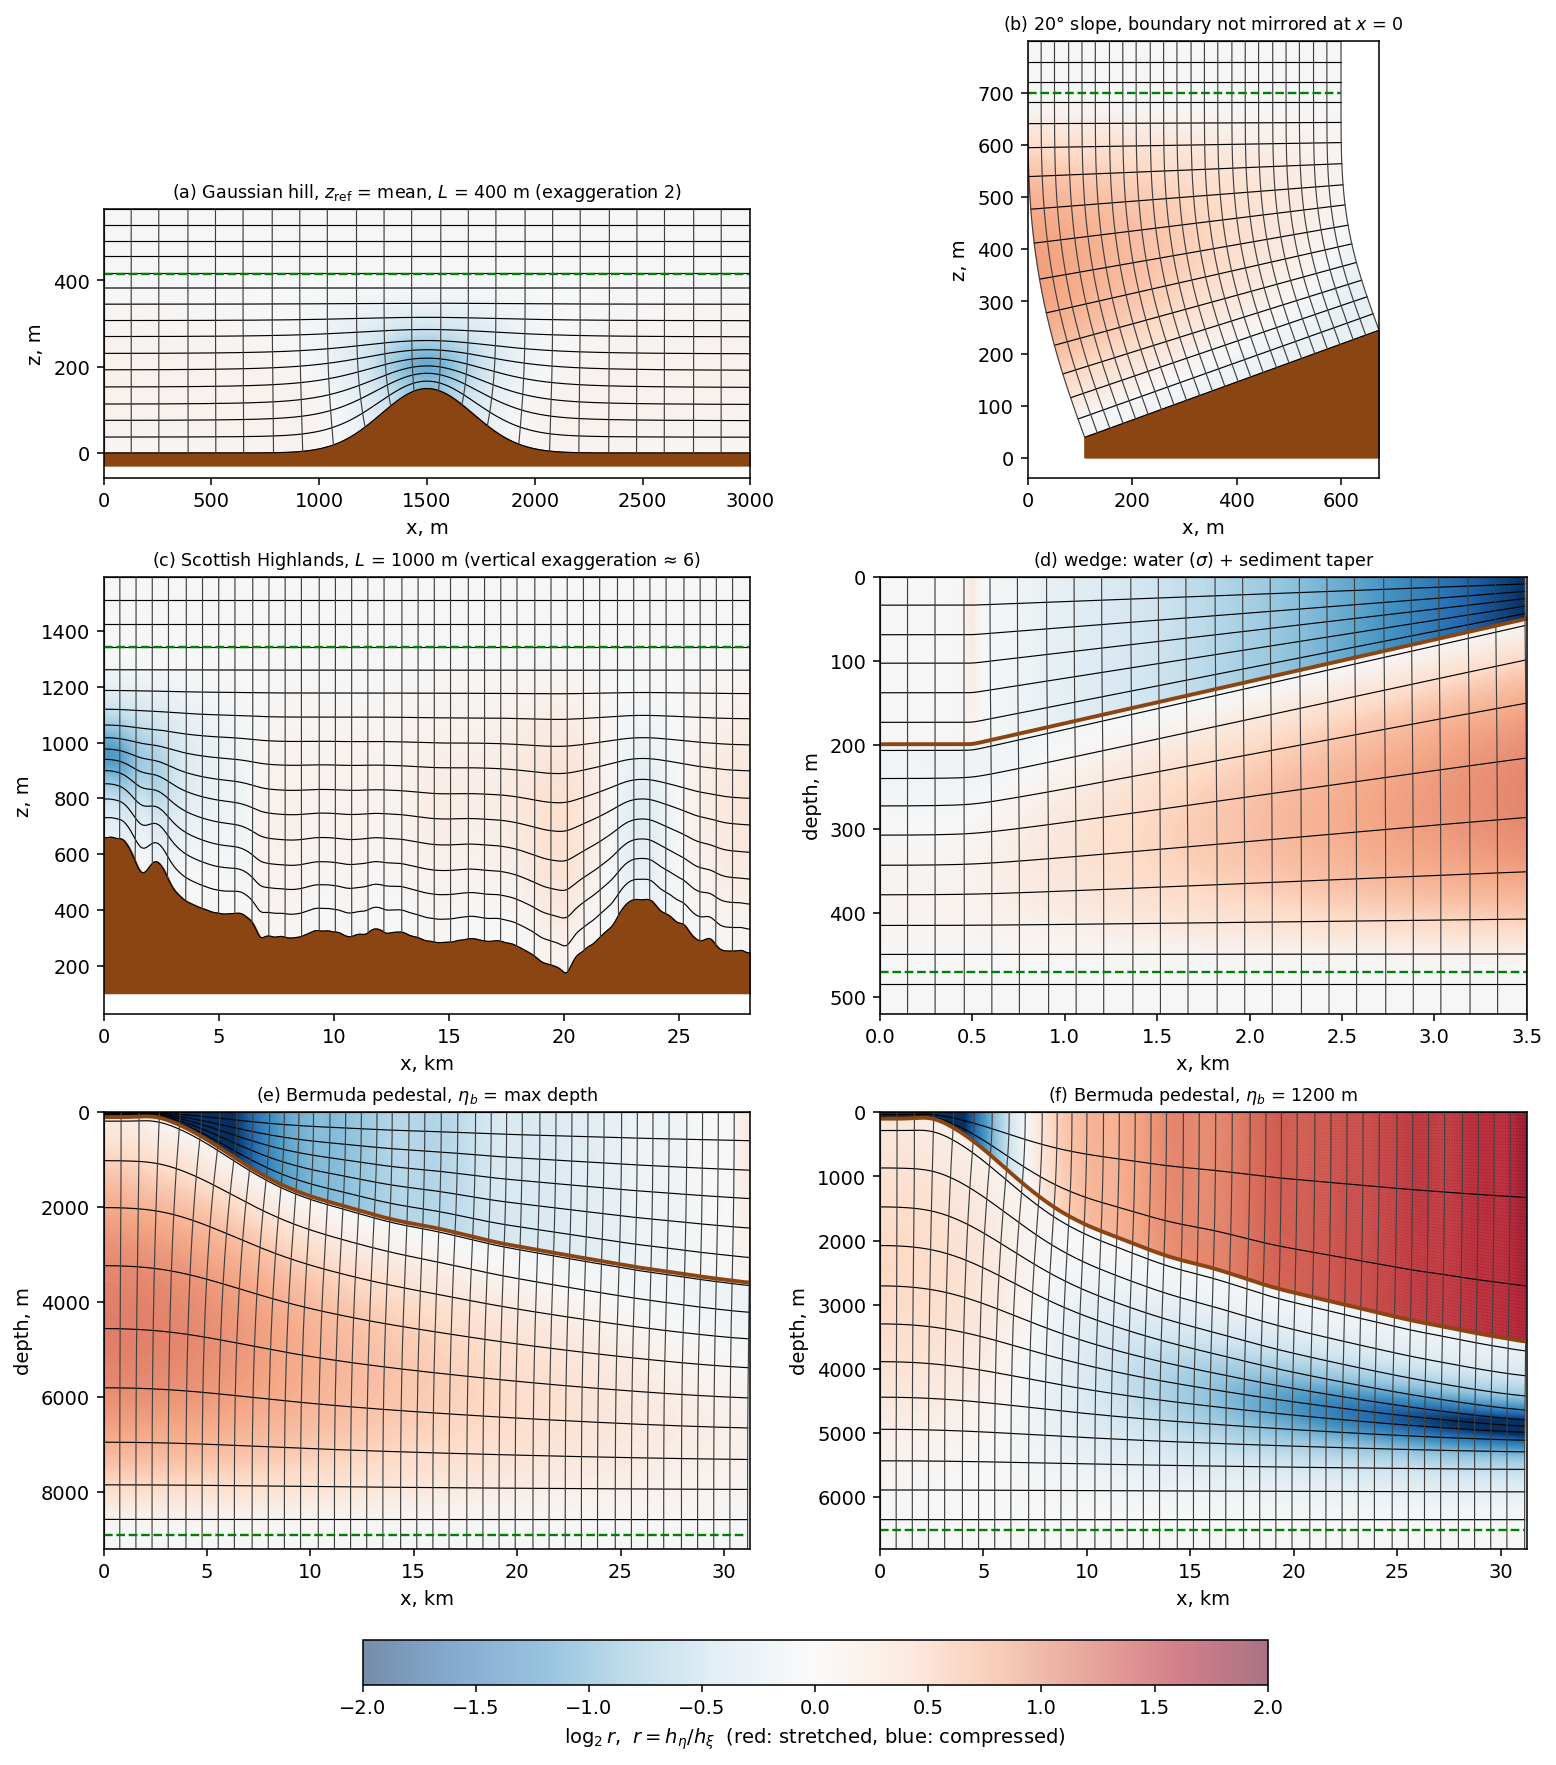
\includegraphics[width=\textwidth]{coordinate_grids.png}
\caption{Orthogonal terrain-following coordinates on examples. Black lines: level
curves $\eta=\mathrm{const}$; grey lines: orthogonal trajectories
$\xi=\mathrm{const}$; colour: $\log_2 r$, $r=h_\eta/h_\xi$; green dashed line: top of
the transition layer $\eta=\etal$, above which the map is the identity; brown line:
seabed $\eta=\etab$. (a)~Gaussian hill: small-scale relief decays over its own
width. (b)~$20^\circ$ slope without the even extension at $x=0$: the starting
trajectory is curved. (c)~Scottish Highlands (\cref{sec:realdata}). (d)~Penetrable
wedge: $\sigma$-coordinates in the water and the tapered extension in the
sediment. (e,f)~Bermuda pedestal with $\etab=\max T$ (strong compression of the
shelf column) and with $\etab=\SI{1200}{m}$ (compression moved into the
sediment, expansion of the deep water). Panels (c)--(f) are vertically
exaggerated, so the right angles appear distorted.}
\label{fig:grids}
\end{figure}

\Cref{fig:grids} shows the resulting coordinates for the examples used
in this note.

%=====================================================================
\section{The transformed one-way equation}\label{sec:transformed}

\subsection{Transformed Helmholtz equation and boundary conditions}

The density depends only on $\eta$ in computational coordinates, because the
seabed is the line $\eta=\etab$. Equation \eqref{eq:helm_orth} holds with:
\begin{itemize}
\item $\psi=0$ at $\eta=0$ (Dirichlet) or $\pd_\eta\psi=0$ (Neumann, since
$\pd_n=h_\eta^{-1}\pd_\eta$);
\item $[\psi]=0$ and $\bigl[(r\rho)^{-1}\pd_\eta\psi\bigr]=0$ at $\eta=\etab$.
\end{itemize}
The latter is equivalent to $[\rho^{-1}\pd_n\psi]=0$ because
$(r\rho)^{-1}\pd_\eta\psi=h_\xi\rho^{-1}\pd_n\psi$ and $h_\xi$ is continuous.

\subsection{Liouville transformation}

Range dependence of $r$ enters through $\pd_\xi(r\rho^{-1}\pd_\xi)$. With
$\psi=r^{-1/2}\varphi$, and using
$\pd_\xi\bigl(r\pd_\xi(r^{-1/2}\varphi)\bigr)=r^{1/2}\varphi_{\xi\xi}-(r^{1/2})_{\xi\xi}\varphi$,
\eqref{eq:helm_orth} becomes
\begin{equation}\label{eq:liouville}
\varphi_{\xi\xi}+B\varphi=0,\qquad
B\varphi=\rho\,r^{-1/2}\pd_\eta\Bigl(\frac{1}{r\rho}\pd_\eta\bigl(r^{-1/2}\varphi\bigr)\Bigr)+\bigl(k^2h_\xi^2-V\bigr)\varphi,\qquad
V=\frac{(r^{1/2})_{\xi\xi}}{r^{1/2}} .
\end{equation}
$B$ is symmetric in $L^2(\rho^{-1}\dd\eta)$. Its range dependence comes only from
the metric and from the medium. $V$ is a curvature-squared term, of relative
size $(\lambda/\ell_\xi)^2$ with respect to $k^2$.

\subsection{Flux-conserving one-way step}

The one-way factorisation of \eqref{eq:liouville} keeps the outgoing part,
$\varphi_\xi=i\sqrt B\varphi-\frac14B^{-1}B_\xi\varphi+\dots$. The second term is
the transport (WKB) term. It expresses the conservation of the energy flux
$\mathcal F=\operatorname{Im}\int\rho^{-1}\bar\varphi\varphi_\xi\,\dd\eta=\|B^{1/4}\varphi\|^2$
instead of $\|\varphi\|^2$. In the standard PE in a slowly range-dependent medium
it is neglected. Here it is not negligible: the coordinate lines rotate with
height, so a beam changes its angle to the local marching direction, and the
plain step $\varphi_{n+1}=\exp(i\Delta\xi\sqrt{B_{n+1/2}})\varphi_n$ preserves
the wrong norm. In the slope tests of \cref{sec:slope} this costs 2--6\,\% of
amplitude over a few hundred metres for beams reflected at $40$--$50^\circ$, in
agreement with the WKB prediction $\bigl(\cos\theta_1/\cos\theta_2\bigr)^{1/2}$
($\theta_{1,2}$ the angles of the beam to the coordinate lines at the two ends).
We use the flux-conserving step
\begin{equation}\label{eq:flux_step}
\varphi_{n+1}=B_{n+1}^{-1/4}\,\exp\bigl(i\Delta\xi\sqrt{B_{n+1/2}}\bigr)\,B_{n}^{1/4}\varphi_n,
\end{equation}
which preserves $\mathcal F$ exactly when the propagator is unitary (cf.\ the
energy-conserving PE \cite{collins1991energy,porter1991energy}, where the same
factors appear at a vertical interface). It is the essential new ingredient of
the scheme; without it the transformation trades the staircase error for an
amplitude drift.

\paragraph{Exterior-identity form.} Since the middle propagator commutes with
$B_{n+1/2}^{\pm1/4}$,
\begin{equation}\label{eq:flux_pairs}
\varphi_{n+1}=\underbrace{\bigl[B_{n+1}^{-1/4}B_{n+1/2}^{1/4}\bigr]}_{C_2}\,
\exp\bigl(i\Delta\xi\sqrt{B_{n+1/2}}\bigr)\,
\underbrace{\bigl[B_{n+1/2}^{-1/4}B_{n}^{1/4}\bigr]}_{C_1}\varphi_n .
\end{equation}
Each bracket is the identity wherever its two columns coincide, in particular in
the whole exterior. The middle factor is the plain rational chain, so the NLBC
\eqref{eq:nlbc} of the plain chain applies unchanged (\cref{sec:nlbc}).

\paragraph{Rational approximation.} With $B=\beta^2(1+L)$, the envelope
$\varphi=e^{i\beta\xi}v$, and the diagonal Pad\'e approximants
$(1+L)^{\pm1/4}\approx\prod_{l=1}^{q}\frac{1+c^\pm_lL}{1+d^\pm_lL}$
($c^-_l=d^+_l$, $d^-_l=c^+_l$; without the rotation introduced below, $q=1$ gives $(1+\frac58L)/(1+\frac38L)$),
\begin{equation}\label{eq:full_step}
v_{n+1}=\prod_{l=1}^{q}\frac{1+c^-_lL_{n+1}}{1+d^-_lL_{n+1}}\prod_{l=1}^{q}\frac{1+c^+_lL_{n+\frac12}}{1+d^+_lL_{n+\frac12}}\;
R(L_{n+\frac12})\;
\prod_{l=1}^{q}\frac{1+c^-_lL_{n+\frac12}}{1+d^-_lL_{n+\frac12}}\prod_{l=1}^{q}\frac{1+c^+_lL_{n}}{1+d^+_lL_{n}}\;v_n .
\end{equation}
\paragraph{Rotated branch cut.} $(1+L)^{1/4}$ has a branch cut on $L<-1$, and its
Pad\'e approximants have their poles and zeros on the cut, i.e.\ inside the
evanescent part of the spectrum of the discrete $L$. The $[2/2]$ approximant
has a pole at $L=-1.38$ and a zero at $L=-1.18$. A pair $C_{1,2}$ at two slightly
different columns is close to the identity, but for an eigenvalue next to a
pole it is not, and it amplifies a spurious evanescent component. With the
$[2/2]$ approximant this produced a localised error of 14\,\% after
\SI{600}{m} in the $20^\circ$ slope test of \cref{sec:slope}. We therefore follow
\cite{milinazzo1997} and approximate
\[
(1+L)^{1/4}=e^{i\gamma/4}\bigl(1+Y\bigr)^{1/4},\qquad Y=(1+L)e^{-i\gamma}-1,
\]
by the $[q/q]$ Pad\'e approximant in $Y$, with $\gamma=45^\circ$. Rewritten as
factors in $L$, its poles and zeros lie at
$L=(1-1/b)e^{i\gamma}-1\notin\mathbb R$, so $|1+bL|$ is bounded away from zero on
the real spectrum. The constant prefactor cancels within each pair. Only the
logarithmic derivative of the approximant enters $C_{1,2}$; for $q=2$ its
relative error is below $5\cdot10^{-2}$ for $L\in[-0.5,0.2]$ (propagation angles up
to $45^\circ$). Since the correction itself is a few per cent of the amplitude,
this gives errors of order $10^{-3}$. With the rotated factors the $20^\circ$
test is accurate to $1.2\cdot10^{-3}$.

\subsection{Factors in terms of the physical field}

All factors in \eqref{eq:full_step} have the form $(1+cL)^{-1}(1+aL)$ with $L$
taken at one column. They are solved for $\psi=r^{-1/2}\varphi$ with $r$ of the
same column, by the following identity.

\begin{lemma}\label{lem:psi_form}
Let $\varphi=r^{1/2}\psi$, $\rt=\rho r$, $m=r^2$ and
$\het=(k^2h_\xi^2-V)/\beta^2-1$. Then
\[
r^{3/2}\beta^2(1+cL)\varphi=\mathcal T_c\psi\equiv c\,\rt\,\pd_\eta\bigl(\rt^{-1}\pd_\eta\psi\bigr)+\beta^2m(1+c\het)\psi .
\]
Hence $(1+bL)\varphi_v=(1+aL)\varphi_u$ if and only if $\mathcal T_b\psi_v=\mathcal T_a\psi_u$.
\end{lemma}
\begin{proof}
$\beta^2(1+cL)\varphi=\beta^2(1-c)\varphi+cB\varphi$. Insert
$B\varphi=\rho r^{-1/2}\pd_\eta\bigl((r\rho)^{-1}\pd_\eta\psi\bigr)+(k^2h_\xi^2-V)r^{1/2}\psi$
and multiply by $r^{3/2}$.
\end{proof}

$\mathcal T_c$ is the operator of the flat density scheme \eqref{eq:substep_flat}
with the density $\rho$ replaced by the generalised density $\rt=\rho h_\eta/h_\xi$
and with the extra weight $m$. Its natural interface conditions,
$[\psi]=0$ and $[\rt^{-1}\psi_\eta]=0$, are the physical ones. Between columns
the field is rescaled by $(r_{\rm old}/r_{\rm new})^{1/2}=(m_{\rm old}/m_{\rm new})^{1/4}$.

%=====================================================================
\section{Discretisation}\label{sec:disc}

\paragraph{Vertical.} On the uniform grid $\eta_j=j\Delta\eta$ every factor of
\eqref{eq:full_step} is
\begin{equation}\label{eq:scheme}
c\,\delta^2_{\rt}v+(1+\alpha\delta^2_{\rt})\bigl[\tau^2m(1+c\het)v\bigr]=a\,\delta^2_{\rt}u+(1+\alpha\delta^2_{\rt})\bigl[\tau^2m(1+a\het)u\bigr],\qquad\tau=\beta\Delta\eta,
\end{equation}
a tridiagonal system. For $r\equiv1$ it is exactly the existing scheme
\eqref{eq:substep_flat}. For smooth $\rt$, with $g=\ln\rt$ and
$D=\rt\pd_\eta\rt^{-1}\pd_\eta$, a Taylor expansion (checked symbolically) gives
\[
\frac{\delta^2_{\rt}}{\Delta\eta^2}=D+\frac{\Delta\eta^2}{12}D^2+\Delta\eta^2E+O(\Delta\eta^4),\quad
E\psi=\tfrac1{24}\bigl(g'^2+g''\bigr)\psi''+\tfrac1{24}\bigl(g'''+g'g''-g'^3\bigr)\psi'.
\]
The Numerov weight cancels the $D^2$ term. The scheme is therefore fourth-order
in the wave part, with an additional second-order error of relative size
$(\Delta\eta/\ell_\eta)^2/24$, where $\ell_\eta$ is the vertical scale of $\ln r$.
In practice $\ell_\eta\gtrsim L\sim10^2\lambda$, so this error is negligible.

\paragraph{Boundary and interface rows.}
\begin{itemize}
\item \emph{Dirichlet.} $v_0=0$ is eliminated from the system rather than
imposed by a unit row: a unit row next to entries $\alpha\tau^2m\gg1$ is
satisfied by a pivoting solver only up to amplified round-off.
\item \emph{Neumann.} Mirror node $v_{-1}=v_1$ with even coefficients.
\item \emph{Seabed node} $j_b=\etab/\Delta\eta$ (a grid node by construction).
The equation is integrated over the cell, so $\rt_{j_b}$ is the harmonic mean of
the one-sided values. $m_{j_b}$ and $\het_{j_b}$ are fixed by
$m_{j_b}/\rt_{j_b}=\langle m/\rt\rangle$ and
$m_{j_b}\het_{j_b}/\rt_{j_b}=\langle m\het/\rt\rangle$, where
$\langle\cdot\rangle$ is the average of the two one-sided values.
\end{itemize}

\paragraph{Range.} The coefficients $\het,m,\rt$ (nodes) and $\rt$ (half-nodes)
are tabulated on coarse columns $\xi_c$ with spacing about $\sigma/4$ (the map
varies on the scale of the smoothed boundary), and only below the identity
region. They are interpolated linearly to $\xi_n$, $\xi_{n+1/2}$, $\xi_{n+1}$.
The main chain is evaluated at the midpoint, which gives second order in the
coefficient variation. The memory is $O(n_c\,\etal/\Delta\eta)$ instead of
$O(n_x n_z)$.

%=====================================================================
\section{Discrete dispersion analysis}\label{sec:dispersion}

Freeze $h_\xi$, $h_\eta$, $\rho$ and $k$ (so $r$, $m=r^2$, $\rt=\rho r$ and $\het$
are constant), and consider an outgoing plane wave with physical angle $\theta$
to the local marching direction: $k_z=k\sin\theta$, computational vertical
wavenumber $q=k_zh_\eta$, and $\psi^n_j=\lambda^ne^{iqj\Delta\eta}$. The flux
factors of \eqref{eq:full_step} cancel ($L_n=L_{n+1/2}=L_{n+1}$). With
$s=\sin^2(q\Delta\eta/2)$, the symbol of \eqref{eq:scheme} gives
\begin{equation}\label{eq:Lh}
L_h(q)=\het-\frac{4}{\tau^2r^2}\,\frac{s}{1-4\alpha s},\qquad\lambda=R\bigl(L_h(q)\bigr),
\end{equation}
while the exact amplification is $e^{i\Delta\xi(p-\beta)}$ with
$p=h_\xi\sqrt{k^2-k_z^2}=h_\xi k\cos\theta$. The dispersion error per unit
physical length is
\begin{equation}\label{eq:disp_err}
\varepsilon(\theta)=\frac{\bigl|\log\bigl(\lambda\,e^{-i\Delta\xi(p-\beta)}\bigr)\bigr|}{h_\xi\Delta\xi}.
\end{equation}

\begin{theorem}[local equivalence]\label{thm:equiv}
$\varepsilon(\theta;\beta,\Delta\xi,\Delta\eta,h_\xi,h_\eta)=\varepsilon_0(\theta;\beta/h_\xi,\,h_\xi\Delta\xi,\,h_\eta\Delta\eta)$,
where $\varepsilon_0$ is the dispersion error of the untransformed scheme
\eqref{eq:substep_flat} with reference wavenumber $\beta/h_\xi$ and steps
$h_\xi\Delta\xi$, $h_\eta\Delta\eta$.
\end{theorem}
\begin{proof}
Let $\beta_e=\beta/h_\xi$, $\Delta x_e=h_\xi\Delta\xi$, $\Delta z_e=h_\eta\Delta\eta$.
\begin{itemize}
\item $\beta\Delta\xi=\beta_e\Delta x_e$, so $R$ has the same coefficients:
those of \eqref{eq:rational} depend on $\beta\Delta x$ only.
\item $\het=k^2h_\xi^2/\beta^2-1=k^2/\beta_e^2-1$.
\item $\tau r=\beta\Delta\eta\,h_\eta/h_\xi=\beta_e\Delta z_e$.
\item $q\Delta\eta=k_z\Delta z_e$.
\end{itemize}
Hence $L_h$ and $\lambda$ coincide. The exact factor is
$e^{i\Delta\xi(h_\xi k\cos\theta-\beta)}=e^{i\Delta x_e(k\cos\theta-\beta_e)}$, and
the normalisations $h_\xi\Delta\xi=\Delta x_e$ agree.
\end{proof}

\begin{figure}[t]\centering
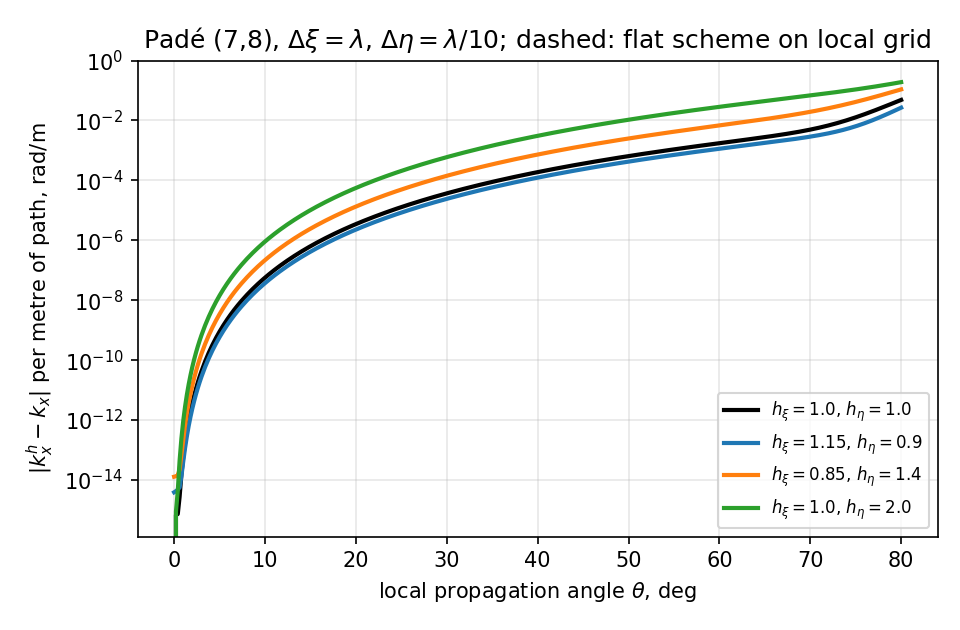
\includegraphics[width=0.49\textwidth]{disp_local_equivalence.png}\hfill
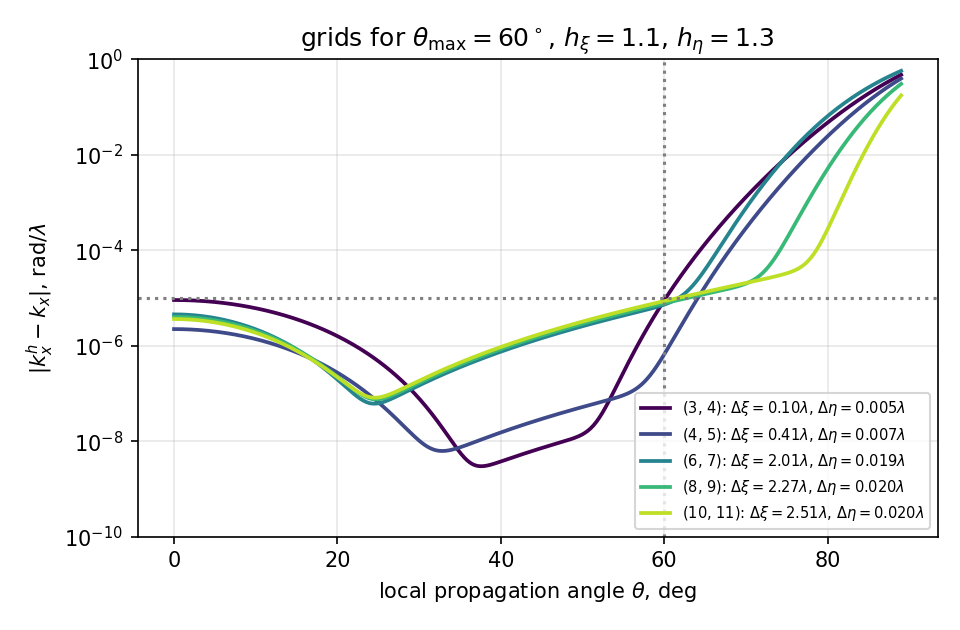
\includegraphics[width=0.49\textwidth]{disp_orders.png}
\caption{Left: dispersion error of the transformed scheme for several metric
values on one grid (solid) and of the untransformed scheme on the local
effective grid (dashed); the curves coincide to $4\cdot10^{-13}$ of the
maximum error, as \cref{thm:equiv} states. Right: Pad\'e orders $(3,4)$--$(10,11)$
on the grids chosen for a $60^\circ$ aperture in a strongly distorted cell
($h_\xi=1.1$, $h_\eta=1.3$); every order reaches the target accuracy up to the
aperture.}
\label{fig:dispersion}
\end{figure}

\Cref{fig:dispersion} confirms \cref{thm:equiv} numerically and shows its
practical meaning.

\begin{corollary}[angles]\label{cor:angles}
The transformation introduces no angle restriction. A wave is resolved if its
angle to the \emph{local} marching direction is within the aperture of the
rational approximation on the local grid. Over terrain with slopes up to
$\theta_s$, waves reflected by the slopes reach $\theta_{\max}+2\theta_s$ to the
horizontal (and to the marching direction above the transition layer), so the
aperture is set to $\min(\theta_{\max}+2\theta_s,85^\circ)$. This requirement
is physical: it applies equally to a staircase, which usually ignores it.
\end{corollary}

\begin{corollary}[grid selection]\label{cor:grid}
Locally the scheme sees $k'=kh_\xi$, $k_z'=k_zh_\xi$, the vertical step
$\Delta z'=r\Delta\eta$ for the operator $r^{-2}\pd^2_\eta$, and the range step
$\Delta\xi$. With $h_\pm=\max/\min h_\xi$, the flat grid optimizer is applied with:
\begin{itemize}
\item the wavenumber interval $[k_{\min}h_-,\ k_{\max}h_+]$;
\item the vertical wavenumber bound $k_z^{\max}h_-$, so that the smallest
longitudinal wavenumber $h_-^2\bigl(k_{\min}^2-(k_z^{\max})^2\bigr)$ is the
pessimistic one;
\item the error budget per unit computational length.
\end{itemize}
The vertical step it returns resolves $k_z^{\max}h_-$. Since the scheme must
resolve $k_z^{\max}h_+$ with the step $r\Delta\eta$, we take
$\Delta\eta=\Delta z'\,(h_-/h_+)/\max r$.
The stability properties of the flat scheme (spectrum of $L_h$ in
$(-\infty,\het]$, $|R|\le1$ there) carry over, because $L_h$ is the flat-scheme
symbol at the local parameters.
\end{corollary}

\begin{remark}[layered media]
In computational coordinates the seabed is a horizontal interface, across which
the longitudinal wavenumber $p$ is conserved. For an aperture $\theta_{\max}$
defined in the water, the field therefore has
$p\ge\min_{\rm water}k\,\cos\theta_{\max}$ in the bottom too. The lower end of
the wavenumber interval is $\min_{\rm water}k$, not the smaller bottom wavenumber;
using the latter would forbid apertures beyond the bottom critical-angle
complement ($\approx64^\circ$ for $1530/1700$\,m/s), although on a downslope
each bottom reflection lowers a ray's angle by $2\theta_s$, so energy beyond the
critical angle can return to long-range paths.
\end{remark}

The remaining errors, which the frozen-coefficient analysis does not see, are:
\begin{enumerate}
\item the coefficient-variation truncation, $O\bigl((\Delta\eta/\ell_\eta)^2\bigr)$;
\item the linear interpolation of the coefficient tables in range, $O\bigl((\Delta\xi_c/\ell_\xi)^2\bigr)$;
\item the one-way (no backscatter) approximation of the range-dependent
operator, which is the same approximation as for any range-dependent medium;
\item the error of the $[q/q]$ approximation of $(1+L)^{\pm1/4}$, which acts on
a quantity that is already of first order in $\Delta\xi\,\pd_\xi\ln B$.
\end{enumerate}
The validation in \cref{sec:slope} bounds them all together: there the field is
accurate to $1.2\cdot10^{-3}$ for a beam reflected at $50^\circ$, and to
$3\cdot10^{-3}$ at $70^\circ$.

%=====================================================================
\section{Compatibility with the upper nonlocal boundary condition}\label{sec:nlbc}

\begin{theorem}\label{thm:nlbc}
Let the computational domain be $0\le\eta\le\eta_{\max}$ with
$\eta_{\max}\ge\etal+2\Delta\eta$, and let the medium in the exterior be
range-independent. Then the discrete NLBC \eqref{eq:nlbc} for the chain
$R=\prod_l(1+a_lL)/(1+b_lL)$, computed for the untransformed exterior scheme, is
the exact discrete transparent boundary condition of the scheme
\eqref{eq:full_step}--\eqref{eq:scheme}.
\end{theorem}
\begin{proof}
\begin{enumerate}
\item In the rows $j\ge\etal/\Delta\eta$ the map is the identity: $h_\xi=h_\eta=r=m=1$,
$V=0$ and $\rt=\rho$. Since the taper is $C^2$, these values hold exactly at the
nodes and half-nodes used by the last rows, so the scheme \eqref{eq:scheme} in
these rows coincides with \eqref{eq:substep_flat} with $z=\eta+z_{\rm off}$.
\item The flux factors are applied as the pairs $C_1$, $C_2$ of
\eqref{eq:flux_pairs}. Each pair is the identity operator in the exterior
because its two columns coincide there. Numerically the pairs are solved on the
rows below $\etal$ plus a margin of four wavelengths, with the top value passed
through, and the rows above are left untouched.
\item What reaches the boundary is therefore produced by the chain $R$ alone,
with exterior coefficients independent of $n$. The derivation of
\cite{lytaev2018awpl} (discrete $z$-transform in range of the exterior
recurrences of the chain) applies verbatim, including the linear-$\het$ (Airy)
exterior.
\end{enumerate}
\end{proof}

\begin{remark}
Writing the flux step as \eqref{eq:flux_step} with the factors placed around $R$
would also be correct. The NLBC would then have to be computed for a chain of
$p+2q$ factors containing reciprocal pairs. The matrix function in the inverse
$z$-transform then becomes defective, and the adaptive quadrature of the kernels
does not converge, which we observed. The form \eqref{eq:flux_pairs} avoids
this, and the NLBC kernels are the same as on flat ground.
\end{remark}

In the ocean the ``upper'' boundary is the bottom of the domain, deep in the
homogeneous sediment. The identity region is reached at depth $\etal=\etab+L$,
so the NLBC sees the homogeneous bottom.

%=====================================================================
\section{Implementation in \texttt{pywaveprop}}\label{sec:impl}

\begin{itemize}
\item \texttt{pywaveprop/terrain\_transform.py}: \texttt{OrthogonalTerrainMap}
(level curves \eqref{eq:family}--\eqref{eq:kernel}, trajectories and metrics
\eqref{eq:traj}--\eqref{eq:metric}; NumPy).
\item \texttt{pywaveprop/helmholtz\_tf\_jax.py}:
\texttt{TerrainFollowingHelmholtzPropagator}, a subclass of
\texttt{RationalHelmholtzPropagator}. It reuses the Pad\'e and
rational-interpolation coefficients, the grid optimizer
(\cref{cor:grid}) and the NLBC kernels, and replaces the vertical operator
by \eqref{eq:scheme} and the range step by \eqref{eq:full_step}. The march is a
\texttt{jax.lax.fori\_loop}.
\item Front-ends: the option \texttt{terrain\_method='transform'} of
\texttt{RWPComputationalParams} (troposphere; Dirichlet or Neumann ground for H
or V polarisation) and of \texttt{UWAComputationalParams} (penetrable seabed
following the bathymetry). The results carry the physical coordinates of the
output nodes.
\end{itemize}

\begin{algorithm}[h]
\caption{One range step of the terrain-following rational propagator}\label{alg:step}
\begin{algorithmic}[1]
\State interpolate $(\het,m,\rt,\rt_{1/2})$ at $\xi_n$, $\xi_{n+1/2}$, $\xi_{n+1}$
\State $\psi\gets C_1\psi$: $q$ factors $\mathcal T_{d^+}^{-1}\mathcal T_{c^+}$ at $\xi_n$; rescale by $(m_n/m_{n+1/2})^{1/4}$; $q$ factors $\mathcal T_{d^-}^{-1}\mathcal T_{c^-}$ at $\xi_{n+1/2}$ \Comment{rows $<\etal$+margin}
\For{$l=1,\dots,p$}
\State solve $\mathcal T_{b_l}\psi'=\mathcal T_{a_l}\psi$ at $\xi_{n+1/2}$ with the NLBC row \eqref{eq:nlbc}; $\psi\gets\psi'$
\EndFor
\State $\psi\gets C_2\psi$ (as in line 2 with $\xi_{n+1/2}\to\xi_{n+1}$)
\end{algorithmic}
\end{algorithm}

\paragraph{Cost.} A step costs $p+4q$ tridiagonal solves. The $4q$ flux solves
are restricted to the transition layer. The coefficient tables add
$O(n_c\etal/\Delta\eta)$ memory. The map is built once, in seconds.

\paragraph{A bug found on the way.} The flat-ground comparison of the new
propagator with the existing one exposed a defect in
\texttt{RationalHelmholtzPropagator}. After the pytree round trip performed by
\texttt{jax.jit}, the zero placeholder of the lower-NLBC kernels switched the lower
NLBC on. The Dirichlet row then read $u_1=0$, so the ground was effectively one
grid step above $z=0$. This is fixed in this work. With the fix the two
propagators agree to $4\cdot10^{-14}$ over flat ground.

%=====================================================================
\section{Validation}\label{sec:validation}

\subsection{Flat ground}
Over flat ground the map is the identity and the terrain-following propagator
reproduces \texttt{RationalHelmholtzPropagator}, including the NLBC, to
$4\cdot10^{-14}$ (unit test \texttt{TestFlatGroundEquivalence}).
\subsection{Exact solution: beam reflected by a perfectly conducting slope}\label{sec:slope}
The incident field is a complex-source-point beam at \SI{300}{MHz}, an exact
solution of the Helmholtz equation, with waist at $(-50,30)$\,m, Rayleigh parameter
\SI{100}{m} and direction $-10^\circ$. Its image in the line $z=x\tan\theta_s$ gives
the exact field above the Dirichlet slope. The reflected beam leaves at
$2\theta_s+10^\circ$, i.e.\ $30$, $50$ and $70^\circ$ for $\theta_s=10$, $20$ and $30^\circ$.
\begin{itemize}
\item Both solvers start from the exact field: on the curved trajectory $\xi=0$
(boundary not mirrored at $x=0$) and on the line $x=0$ respectively.
\item Both use Pad\'e $(7,8)$, the aperture $\theta_{\max}=10^\circ+2\theta_s+5^\circ$
and grids chosen by the respective optimizers.
\item The error is $\max|u-u_{\rm exact}|/\max|u_{\rm exact}|$ over the computational
domain above the ground.
\end{itemize}
\begin{table}[h]\centering
\caption{Exact slope test (Pad\'e $(7,8)$, precision parameter $10^{-2}$).}\label{tab:slope}
\begin{tabular}{rrrrrrrr}\toprule
& & \multicolumn{3}{c}{terrain-following} & \multicolumn{3}{c}{staircase}\\
\cmidrule(lr){3-5}\cmidrule(lr){6-8}
$\theta_s$ & aperture & $\Delta x$, m & $\Delta z$, m & error & $\Delta x$, m & $\Delta z$, m & error\\\midrule
$10^\circ$ & $35^\circ$ & 2.50 & 0.0345 & $1.4\cdot10^{-4}$ & 2.50 & 0.0625 & $5.4\cdot10^{-1}$\\
$20^\circ$ & $55^\circ$ & 2.50 & 0.0192 & $1.2\cdot10^{-3}$ & 2.50 & 0.0345 & $6.9\cdot10^{-1}$\\
$30^\circ$ & $75^\circ$ & 1.00 & 0.0093 & $2.9\cdot10^{-3}$ & 1.00 & 0.0159 & $8.1\cdot10^{-1}$\\
\bottomrule\end{tabular}\end{table}
\begin{figure}[t]\centering
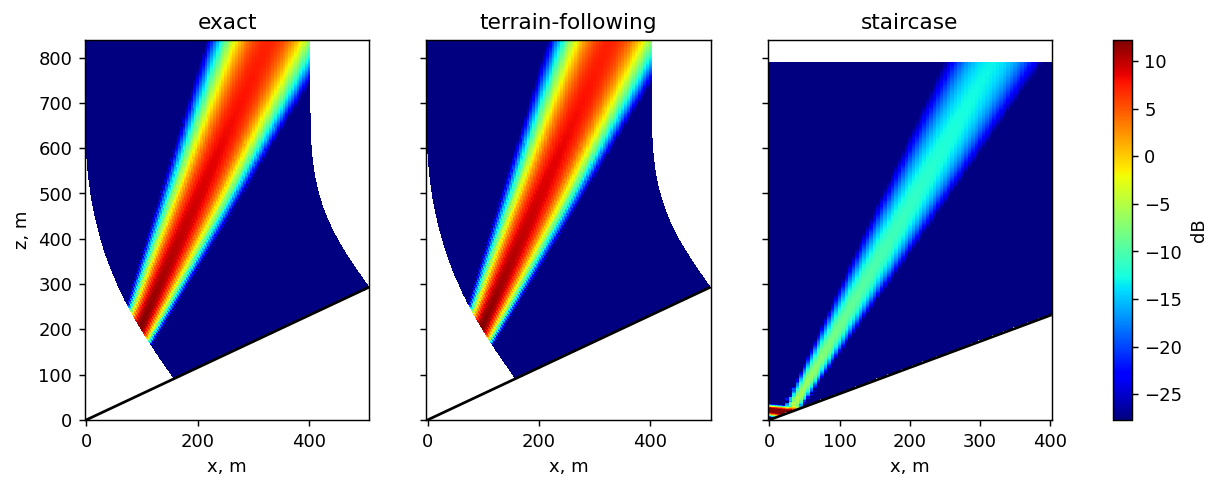
\includegraphics[width=\textwidth]{slope_exact_30deg_maps.png}\\
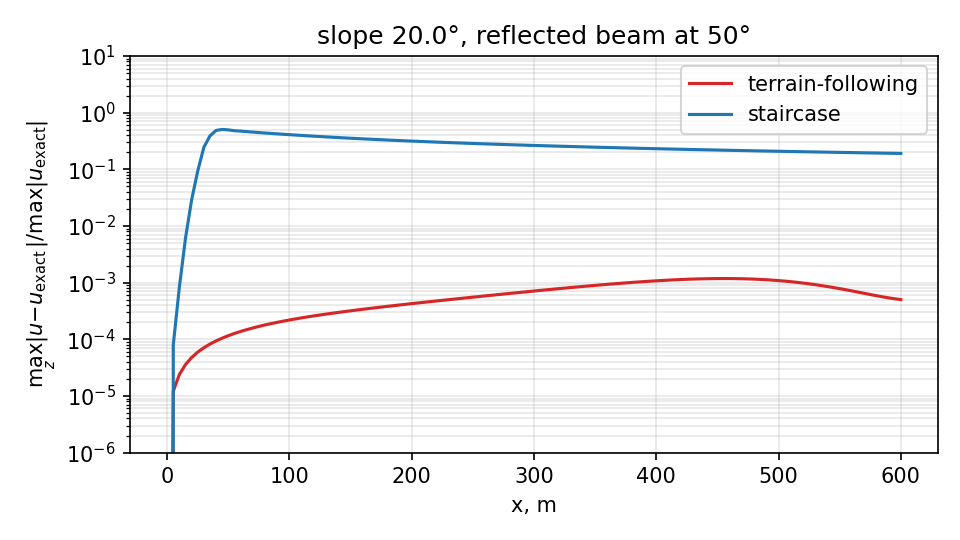
\includegraphics[width=0.49\textwidth]{slope_exact_20deg_error.png}\hfill
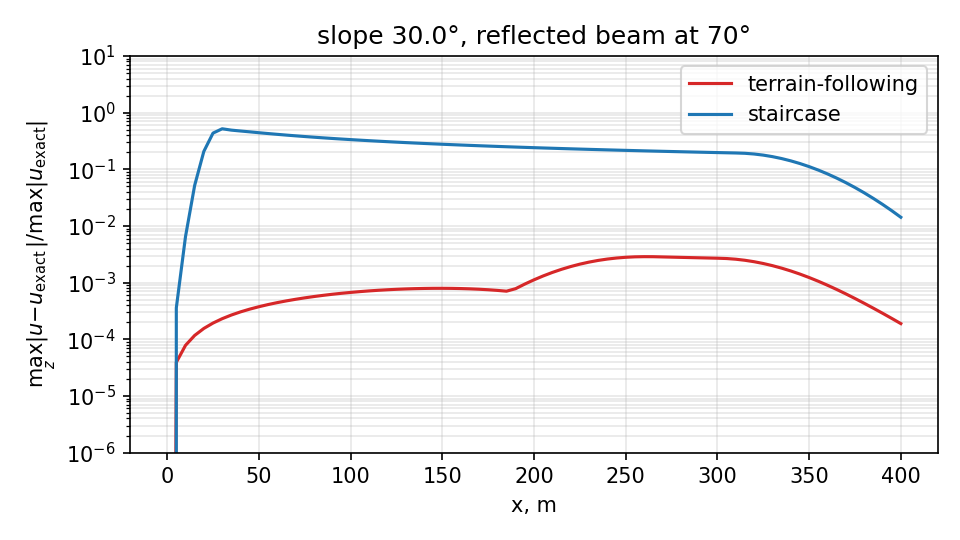
\includegraphics[width=0.49\textwidth]{slope_exact_30deg_error.png}
\caption{Beam reflected by a perfectly conducting slope. Top: $|u|$ for
$\theta_s=30^\circ$ (reflected beam at $70^\circ$); the terrain-following domain is
bounded by the curved trajectories $\xi=0$ and $\xi=x_{\max}$. Bottom: error versus
range for $\theta_s=20^\circ$ and $30^\circ$.}\label{fig:slope}
\end{figure}
The terrain-following error (\cref{tab:slope}, \cref{fig:slope}) is
$10^{-4}$--$3\cdot10^{-3}$ up to a reflected beam at $70^\circ$, on grids
comparable to those of the staircase. The staircase loses most of the reflected
beam, and its error is $0.5$--$0.8$. Refining the staircase grid for $\theta_s=20^\circ$ to
$\Delta z=0.005$\,m ($\lambda/200$) leaves the error at 0.54, and with
$\Delta x=0.625$\,m it is still 0.45: the staircase error is
geometric and decreases only slowly.

The flux-conserving step is essential:
\begin{itemize}
\item With the Liouville rescaling alone ($q=0$) the error in the $20^\circ$ case is
$6.4\cdot10^{-2}$, an amplitude drift along the reflected beam. Without the
rescaling it is larger still.
\item With unrotated $[2/2]$ factors a spurious evanescent component grows to
$0.14$ (\cref{sec:transformed}).
\item The rotated factors give $1.2\cdot10^{-3}$.
\end{itemize}
\subsection{Penetrable wedge}
The upslope wedge of the ASA benchmark \cite{jensen1990benchmark} has the
following parameters:
\begin{itemize}
\item \SI{25}{Hz}, water $c=\SI{1500}{m/s}$;
\item bottom \SI{1700}{m/s}, $\rho=1.5$, \SI{0.5}{dB/\lambda};
\item source at \SI{100}{m};
\item depth \SI{200}{m} with a flat lead-in to \SI{500}{m}, then a $2.86^\circ$ upslope to \SI{3.5}{km}.
\end{itemize}
All solvers use the same smoothed bathymetry ($\sigma=\SI{20}{m}$) and start from
the self-starter of RAM~1.5 at $r=\SI{1}{m}$; a patched copy of RAM writes it out.
RAM is single precision. On fine grids its tridiagonal systems lose all
accuracy: at $\Delta r=\SI{1}{m}$, $\Delta z=\SI{0.05}{m}$ the field is wrong by
\SI{77}{dB}. We therefore rebuilt it in double precision. It then converges: the
grids $(2.5,0.1)$\,m and $(1,0.025)$\,m differ by \SI{0.013}{dB} (median),
and the latter is the reference.
\begin{table}[h]\centering
\caption{Penetrable wedge: median / 90th percentile of $|\Delta\mathrm{TL}|$ (dB) with
respect to the RAM reference, $r>\SI{200}{m}$.}\label{tab:wedge}
\begin{tabular}{lcc}\toprule
solver (grid) & $z=\SI{30}{m}$ & $z=\SI{150}{m}$\\\midrule
terrain-following ($\Delta x=5$, $\Delta z=0.5$\,m) & 0.05 / 0.22 & 0.13 / 0.33\\
same scheme, stair-step bottom ($\Delta x=5$, $\Delta z=1.0$\,m) & 0.54 / 1.29 & 0.82 / 2.07\\
RAM ($\Delta r=10$, $\Delta z=0.5$\,m) & 1.66 / 6.70 & 2.79 / 10.42\\
\bottomrule\end{tabular}\end{table}
\begin{figure}[t]\centering
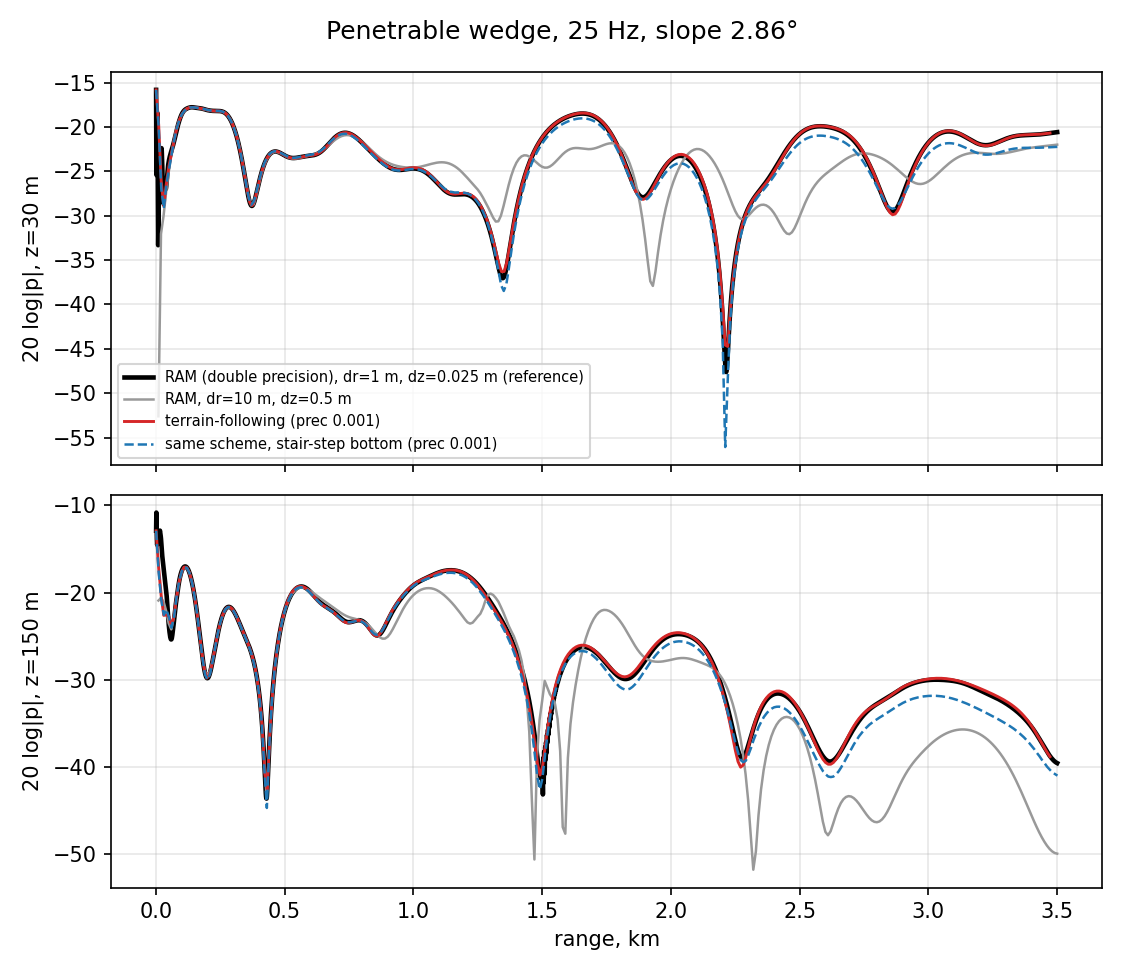
\includegraphics[width=0.66\textwidth]{wedge_uwa_25hz_cuts.png}\hfill
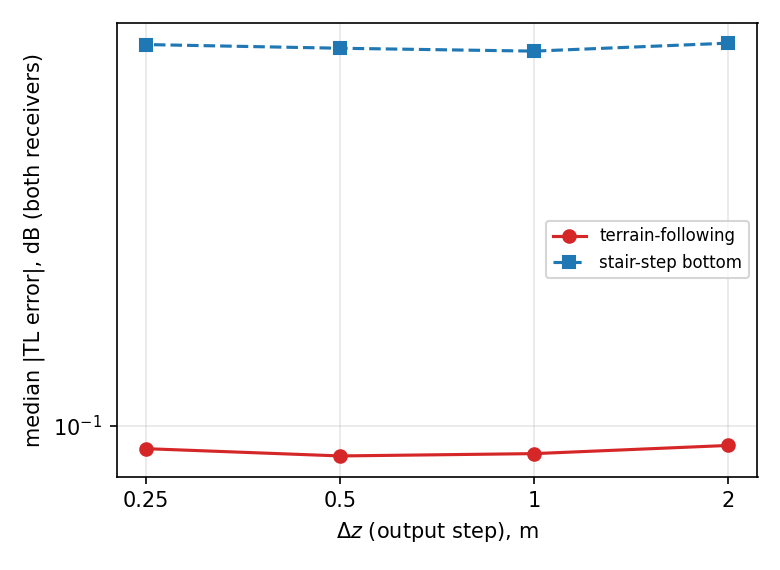
\includegraphics[width=0.33\textwidth]{wedge_uwa_25hz_convergence.png}
\caption{Penetrable wedge. Left: $20\log|p|$ at \SI{30}{m} and \SI{150}{m} depth.
Right: median error versus $\Delta z$ at the same range step.}\label{fig:wedge}
\end{figure}
The terrain-following solution agrees with the reference to
0.05--0.13\,dB (\cref{tab:wedge},
\cref{fig:wedge}). The stair-step bottom in the same scheme gives
0.5--0.8\,dB.

Refining $\Delta z$ from 2 to \SI{0.25}{m} does not reduce either error
(terrain-following 0.09--0.09\,dB, stair-step
0.68--0.71\,dB), and neither does refining
$\Delta x$ to \SI{1.25}{m} or raising the flux order to $q=3$. The two floors have
different origins:
\begin{itemize}
\item \emph{Stair-step.} This is the energy-conservation defect of one-way models
across vertical density steps \cite{porter1991energy}. Each step makes an error
$O(\Delta h)$ and there are $O(1/\Delta h)$ steps, so the bias does not vanish.
RAM avoids it through its density-scaled variable.
\item \emph{Terrain-following.} The residual of about \SI{0.1}{dB} is the
difference between two one-way models of the same sloping interface (RAM's
stair-steps, ours continuous). It is grid-independent. It is larger at the
receiver that lies in the sediment beyond \SI{1.5}{km}.
\end{itemize}


%=====================================================================
\section{Real-world demonstrations}\label{sec:realdata}

\subsection{Troposphere: Scottish Highlands, GFS refractivity}
The path runs from \ang{57.2163}N \ang{4.9214}W (top of a \SI{664}{m} ridge) to
\ang{57.40}N \ang{4.60}W (\SI{28}{km}). The data are:
\begin{itemize}
\item elevation tiles of \texttt{pywaveprop.environment} at \ang{0.0005} resolution
(terrain from 166 to \SI{664}{m}, smoothed with $\sigma=\SI{100}{m}$, maximum slope
$11.1^\circ$);
\item the modified refractivity of the GFS analysis 2026-10-09T12:00Z interpolated
along the path and averaged over range (\cref{fig:tropo}, right).
\end{itemize}
A \SI{300}{MHz} H-polarised antenna on a \SI{30}{m} mast (beam $4^\circ$, tilted
$1^\circ$ down) radiates over perfectly conducting ground. The aperture is
$5^\circ+2\cdot11.1^\circ=27.3^\circ$
(\cref{cor:angles}) for both solvers, and the staircase solver sees the same
smoothed terrain.
Path loss \SI{10}{m} above the ground (median / 90th percentile of the difference):
\begin{itemize}
\item the two precision settings of the terrain-following solver differ by
0.08 / 0.17\,dB;
\item those of the staircase solver differ by 0.15 / 0.48\,dB;
\item the two solvers at the finer setting differ by 1.09 /
3.04\,dB (at \SI{50}{m}: 0.44 / 1.35\,dB).
\end{itemize}
Each solver is thus converged with respect to its own grid; the two agree to
about \\SI{1}{dB} (median) \\SI{10}{m} above the ground and \\SI{0.4}{dB} at
\\SI{50}{m}. The largest differences, up to a few
decibels, occur on the slopes facing the transmitter (21--23\,km and the first
kilometres). There the staircase solution carries small-scale ripple that the
smooth-boundary solution does not, consistent with scattering by the steps
(\cref{sec:slope}).
Run times: terrain-following 468 and 1390\,s,
staircase 73 and 117\,s.
\begin{figure}[t]\centering
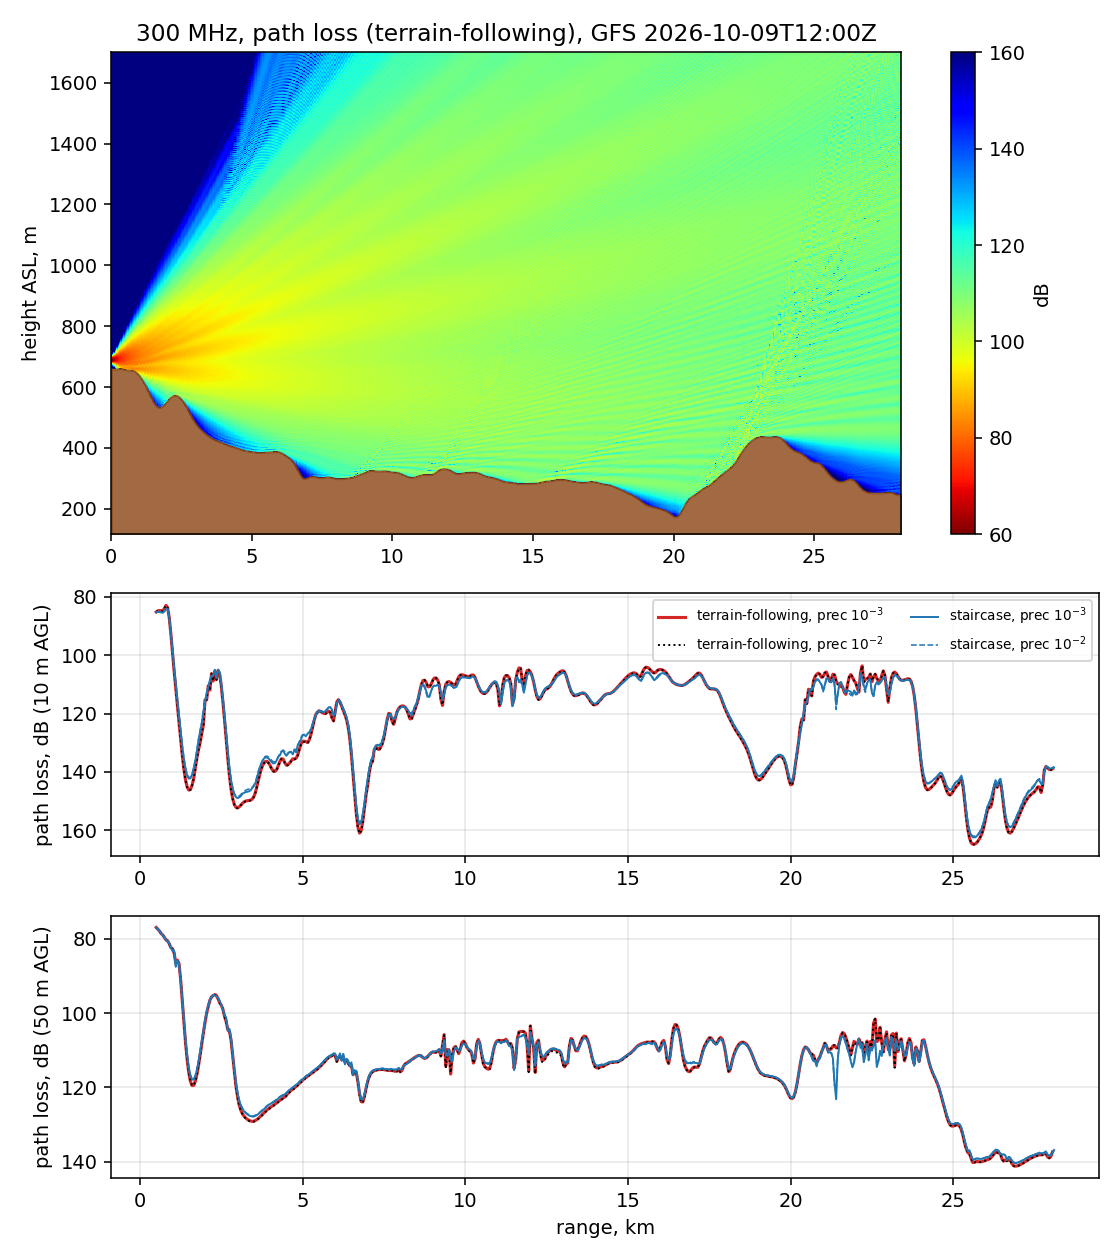
\includegraphics[width=0.74\textwidth]{troposphere_highlands.png}\hfill
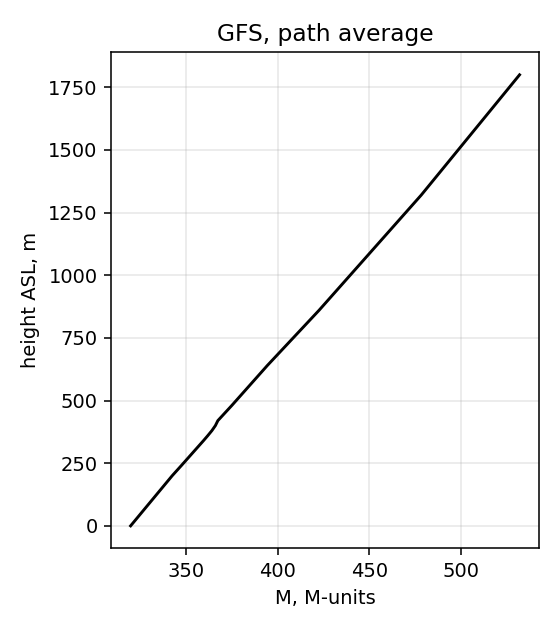
\includegraphics[width=0.25\textwidth]{troposphere_highlands_M.png}
\caption{Scottish Highlands, \SI{300}{MHz}. Path loss of the terrain-following
solver (top), path loss \SI{10}{m} and \SI{50}{m} above the ground for both solvers
and two precision settings, and the GFS M-profile.}\label{fig:tropo}
\end{figure}
\subsection{Underwater acoustics: Bermuda pedestal, Argo sound speed}
The path runs from \ang{32.475}N \ang{64.598}W (\SI{100}{m} deep, on the
edge of the Bermuda platform) to \ang{32.70}N \ang{64.40}W (\SI{3400}{m}).
The data are:
\begin{itemize}
\item bathymetry from the elevation tiles at \ang{0.002} (smoothed with
$\sigma=\SI{500}{m}$, maximum slope $16.1^\circ$);
\item the mean Argo sound speed profile of the area (2020--2023) to \SI{2000}{m},
extended with the deep isothermal gradient \SI{0.0165}{s^{-1}};
\item a fluid bottom (\SI{1700}{m/s}, 1.5, \SI{0.5}{dB/\lambda}) whose interface
follows the bathymetry.
\end{itemize}
A \SI{100}{Hz} source \SI{50}{m} deep radiates down the slope. All solvers start
from RAM's self-starter. The terrain-following domain extends to
\SI{9063}{m}, and the NLBC lies in the homogeneous bottom. The
reference is double-precision RAM at $\Delta r=\SI{2.5}{m}$,
$\Delta z=\SI{0.125}{m}$; RAM at $(5, 0.25)$\,m differs from it by
0.11--0.14\,dB (median).
\begin{table}[h]\centering
\caption{Bermuda pedestal: median / 90th percentile of $|\Delta\mathrm{TL}|$ (dB) with
respect to RAM ($\Delta r=2.5$, $\Delta z=0.125$\,m), $r>\SI{500}{m}$.}\label{tab:bermuda}
\begin{tabular}{llcc}\toprule
aperture & solver (grid) & $z=\SI{50}{m}$ & $z=\SI{500}{m}$\\\midrule
$70^\circ$ & terrain-following ($\Delta x=5.0$, $\Delta z=0.29$\,m) & 0.68 / 2.04 & 0.74 / 4.54\\
$70^\circ$ & stair-step ($\Delta x=5.0$, $\Delta z=0.67$\,m) & 0.42 / 0.89 & 0.59 / 2.86\\
-- & RAM ($\Delta r=5$, $\Delta z=0.25$\,m) & 0.11 / 0.40 & 0.14 / 1.04\\
\bottomrule\end{tabular}\end{table}
\begin{figure}[t]\centering
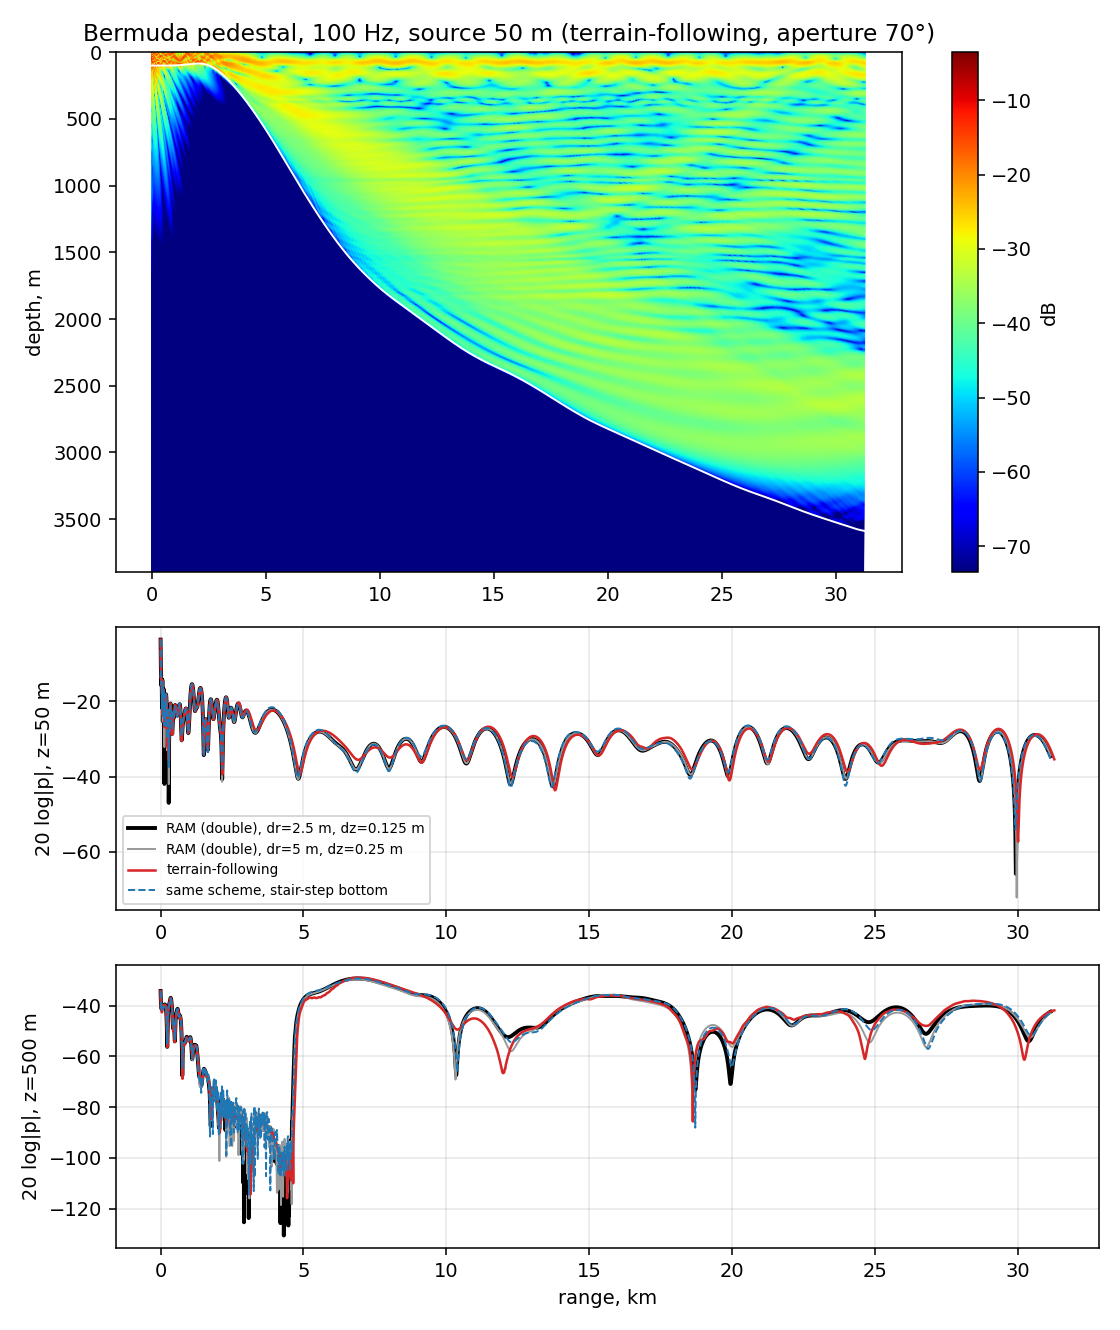
\includegraphics[width=0.8\textwidth]{underwater_bermuda_70deg.png}
\caption{Bermuda pedestal, \SI{100}{Hz}: field of the terrain-following solver
($70^\circ$ aperture) and $20\log|p|$ at \SI{50}{m} and \SI{500}{m} depth.}\label{fig:bermuda}
\end{figure}
With a $70^\circ$ aperture (\cref{tab:bermuda}, \cref{fig:bermuda}) the
terrain-following solution differs from the RAM reference by
0.68 and 0.74\,dB (median at 50 and
\SI{500}{m}); the stair-step bottom gives 0.42 and
0.59\,dB.

The difference is not a discretisation error:
\begin{itemize}
\item halving $\Delta x$ changes it by \SI{0.03}{dB} (0.69/0.74 $\to$ 0.65/0.71\,dB);
\item raising the flux order to $q=3$ changes it by less than \SI{0.02}{dB} (0.66/0.70\,dB);
\item lowering $\etab$ from \SI{3600}{m} to \SI{1200}{m} reduces it to 0.54/0.65\,dB.
\end{itemize}
With $\etab=\max T$ the $\sigma$-map compresses the \SI{100}{m} shelf column 36 times, so $r$ jumps by a factor of about 30 across the seabed. Part of the
difference is therefore the second-order treatment of this extreme interface
row, and a less compressive choice of $\etab$ is preferable for large depth
contrasts. The remainder is of the same order as the difference between the two
stair-step solvers (ours and RAM). Over a \ang{16} penetrable slope, RAM is
itself a stair-step one-way model, and we have no exact reference to say which
one-way treatment is closer to the full solution. The exact test of
\cref{sec:slope} and the wedge of \cref{tab:wedge} are the discriminating
cases.
Times: terrain-following 273\,s, stair-step 966\,s, RAM
27\,s and 97\,s.


%=====================================================================
\section{Conclusions and limitations}\label{sec:conclusions}

Orthogonal terrain-following coordinates, built from the tapered harmonic
extension of the boundary and its orthogonal trajectories, turn terrain and
bathymetry into a generalised density and a weight in the Numerov scheme. The
rational propagator, of any order and with the angle limit of the flat scheme on
the local grid (\cref{thm:equiv}), and the discrete NLBC (\cref{thm:nlbc}) are
used without modification. The essential additional ingredient is the
flux-conserving step \eqref{eq:flux_pairs}. Without it a beam whose angle to the
coordinate lines changes loses amplitude.

\paragraph{Limitations and open points.}
\begin{itemize}
\item \emph{Finite-impedance ground over terrain.} The angle-dependent lower NLBC
of \cite{lytaev2022radarconf} assumes a range-independent boundary row; over
terrain the boundary coefficients depend on $\xi$. A local Leontovich condition
($\pd_\eta\psi+ik\varsigma h_\eta\psi=0$) is straightforward. An exact
angle-dependent condition with range-dependent coefficients is open.
\item \emph{Boundary smoothing.} The boundary has to be $C^2$; corners (knife
edges, cliffs, vertical walls) are smoothed over the scale $\sigma$. Very steep
or overhanging relief makes $Z_\eta$ small and requires a large transition
height $L$.
\item \emph{Range-dependent refractivity.} The exterior has to be
range-independent, exactly as for the flat NLBC. Inside the transition layer a
range-dependent medium is admissible: the tables are per column.
\item \emph{Global metric bounds.} The grid is selected with the extreme values
of $h_\xi$ and $r$ over the whole domain (\cref{cor:grid}). Over strongly
distorted maps (the Bermuda pedestal: $h_\xi\in[0.87,1.27]$) this widens the
wavenumber interval of the rational approximation considerably and limits the
feasible aperture. A range-dependent choice of $\Delta\eta$ is not possible (the
grid is fixed), but a local check of the error budget, or a map that minimises
the spread of $h_\xi$, would reduce the pessimism.
\item \emph{Large depth contrast in the strip map.} With $\etab=\max T$ the
$\sigma$-coordinates compress a shallow column by $T_{\min}/\max T$. On the Bermuda
pedestal this factor is $1/36$, so $r$ jumps strongly across the seabed node. A
smaller $\etab$ reduces the jump at the price of a larger $\max r$ (finer
$\Delta\eta$). A near-conformal profile with guaranteed $Z_\eta>0$, or a
higher-order interface row, would remove the trade-off.
\item The starting field is prescribed on the trajectory $\xi=0$, which is
vertical when the boundary is extended evenly at $x=0$; otherwise it has to be
given on a curve.
\end{itemize}

\bibliographystyle{unsrtnat}
\bibliography{refs/refs}

\end{document}
